% !TeX TS-program = xelatex
% This is SJTUBeamermin v1.0
% For more detailed desciption, see
% https://github.com/LogCreative/SJTUBeamermin/blob/main/doc/sjtubeamermintheme.pdf
%
\documentclass[
    % draft,                             % 草稿模式
    aspectratio=169,                   % 使用 16:9 比例
]{beamer}
\mode<presentation>
\usetheme[
    navigation=subsections,            % 使用子章节进度显示
     lang=en,                           % 使用英文
    % cjk=true,                          % 使用CJK而不是ctex
    color=blue,                         % 使用红色主题
    % pattern=all,                        % 使用全图案装饰
    % gbt=bibtex,                        % 使用 gbt (使用 bibtex 编译)
]{sjtubeamermin}
% \usecolortheme[]{beaver}                 % 使用其他颜色主题
% \addbibresource{ref.bib}               % gbt!=bibtex

\usepackage{amsmath,amsthm}
\usepackage{bm}
\usepackage{tikz-cd}
\usepackage{tikz}
\usetikzlibrary{trees}
\usepackage{empheq}
\usepackage{tabularx}
\usepackage{pifont}
\usepackage{multicol}
\usepackage[linesnumbered,ruled]{algorithm2e}
\usepackage{hyperref}
\usepackage{amsfonts}
\usepackage{tasks}
\usepackage{fontspec}
\usepackage{mdframed} % Add easy frames to paragraphs
\usepackage{color,soul}
\usepackage{xparse} % Add support for \NewDocumentEnvironment

\usepackage[customcolors]{hf-tikz}
\tikzset{style green/.style={
    set fill color=green!50!lime!60,
    set border color=white,
  },
  style cyan/.style={
    set fill color=cyan!90!blue!60,
  },
  style orange/.style={
    set fill color=orange!80!red!60,
  },
  hor/.style={
    above left offset={-0.31,0.31},
    below right offset={0.31,-0.2},
    #1
  },
  ver/.style={
    above left offset={-0.1,0.3},
    below right offset={0.15,-0.15},
    #1
  }
}

\renewcommand{\Bbb}{\mathbb}
\newcommand{\Z}{\mathbb{Z}}
\newcommand{\GR}{\mathbb{GR}}
\newcommand{\F}{\mathbb{F}}
\newcommand{\R}{\mathbb{R}}
\newcommand{\Fns}{\mathbb{F}_{2^n}^*}
\newcommand{\Fn}{\mathbb{F}_{2^n}}
\newcommand{\Fks}{\mathbb{F}_{2^k}^*}
\newcommand{\Fk}{\mathbb{F}_{2^k}}
\newcommand{\df}{\delta_F}
\newcommand{\tr}{\operatorname{tr}_1^k}
\newcommand{\gtr}{\operatorname{T}}
\newcommand{\Bn}{\mathcal{B}_n}
% The symbol of sharing
\newcommand{\Sh}{\operatorname{Sh}}
% The symbol of Teichmuller sets
\newcommand{\teich}{\textit{Teichm$\ddot{u}$ller sets}}

% \newtheorem*{definition}{Definition}
\newtheorem{thm}{Theorem}
\newtheorem{lem}[thm]{Lemma}
\newtheorem{proposition}{Proposition}
\definecolor{graylight}{cmyk}{.30,0,0,.67} % define color using xcolor syntax
\setbeamertemplate{itemize items}[default]

% modify the footnote symbol 
% \makeatother
% \renewcommand{\thefootnote}{\ifcase\value{footnote}\or\dagger\or(\#\#)\or(\#\#\#)\or(\#\#\#\#)\or(\#\#\#\#\#)\fi}
% \makeatletter



\newmdenv[ % Define mdframe settings and store as leftrule
  linecolor=red,
  topline=false,
  bottomline=false,
  rightline=false,
  skipabove=\topsep,
  skipbelow=\topsep
]{leftrule}

% \NewDocumentEnvironment{example}{O{\textbf{Example:}}} % Define example environment
% {\begin{leftrule}\noindent\textcolor{blue}{#1}\par}
% {\end{leftrule}}
\setbeamertemplate{footline}[frame number]

\NewDocumentEnvironment{question}{O{\textbf{Something:}}} % Define something environment
{\begin{leftrule}\noindent\textcolor{graylight}{#1}\par}
{\end{leftrule}}

\NewDocumentEnvironment{remark}{O{\textbf{Remark:}}} % Define remark environment
{\begin{leftrule}\noindent\textcolor{blue}{#1}\par}
{\end{leftrule}}

\begin{document}
    \institute[School of Electronic Information and Electrical Engineering]{电子信息与电气工程学院}   % 组织
    % \logo{
    %     
\includegraphics{support/cnlogored.pdf}  % 重定义 logo
    % }
    \titlegraphic{                         % 标题图像
        \begin{stampbox}[white]
            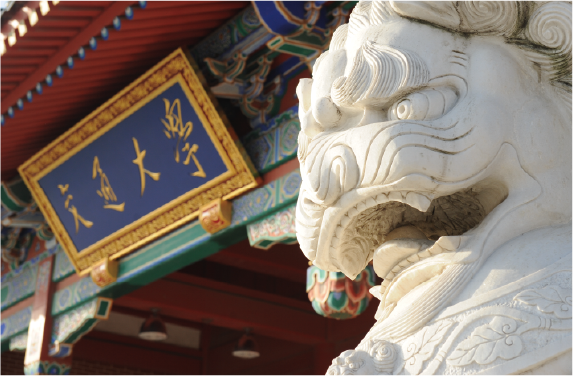
\includegraphics[width=0.3\textwidth]{support/head.png}
        \end{stampbox}
    }
    \title{Threshold Implementations of Bijective S-boxes}  % 标题
 %   \subtitle{SJTUBeamer \fbox{\textsc{min}} Template}         % 副标题
    \author{Zhaole Li}                  % 作者
    \date{\textcolor{red}{2022/12/21}}                          % 日期
    \maketitle                             % 创建标题页


\AtBeginSection[]{
   \begin{frame}
       % \tableofcontents[currentsection]           % 传统节目录             
       \sectionpage                   % 节页
   \end{frame}
}

% 使用小节目录
%\AtBeginSubsection[]{                  % 在每小节开始
 %   \begin{frame}
        % \tableofcontents[currentsection,currentsubsection]             % 传统小节目录             
  %      \subsectionpage                % 小节页
 %   \end{frame}
%}

% \section{Introduction}
%\subsection{第 1 小节}
    \begin{frame}
        \frametitle{Differential Power Analysis}
        \begin{itemize}
            \item Side-channel attacks exploit information that leaks from cryptographic devices 
            and power analysis is one form of those attacks.
            \item Power analysis uses a physical device's power consumption that maybe leak some information to derive secret keys.
            \item Differential power analysis and simple power analysis are two main approaches.
            \item `Differential' means finding the difference between two results of the intermediates in a cryptographic calculation, 
            for example, for the least-significant bit (LSB) of the S-box in AES in round $ 1 $, the difference 
            of results when LSB was $ 1 $ and LSB was $ 0 $. 
        \end{itemize}

    \end{frame}

    \begin{frame}
        \frametitle{Masking}
        \begin{itemize}
            \item To against DPA attacks, a commonly used approach is to make the intermediate results of algorithms executing independent with the secret keys by randomizing all intermediate results.
            \item One of the most widely used techniques to secure an implementation is secret sharing, 
            as known as masking.
            \item In $ s $-share sharing, a variable $ x\in\F_{2^n} $ is shared as $ s $ values 
            $ \left( x_1,...,x_s \right)\in\F_{2^n}^s $.
            \item However, glitches that occur in the masked S-boxes also lead to a side-channel leakage.  
        \end{itemize}
    \end{frame}

    \begin{frame}
        \frametitle{Threshold Implementations (TI)}
    
        Threshold Implementations, a methodology to against DPA attacks and glitches, add two properties over 
        the regular sharing, non-complete and uniform.
        
        Let $ z=N(x,y,...) $ denote a transformation over $ \F_{2^n} $ 
        and we consider input $ s $-sharing $ x_1,x_2,\dots,x_s,y_1,y_2,\dots,y_s,\dots $ 
        and output $ t $-sharing $ z_1,z_2,\dots,z_t $. 

        
    \end{frame}
    \begin{frame}
        \frametitle{Non-completeness in Threshold Implementations (TI)}
        
        We say a sharing of function $ z=N(x,y,...) $ is non-complete, 
        if every function $ z_i $ is independent of at least one share of each of the input variables $ x,y,... $.

        For example, when $ s=t $, we have 
        \begin{align*}
            z_1&=f_1(x_2,\dots,x_s,y_2,\dots,y_s,\dots)\\
            z_2&=f_1(x_1,x_3,\dots,x_s,y_1,y_3,\dots,y_s,\dots)\\
            &\vdots\\
            z_s&=f_1(x_1,\dots,x_{s-1},y_1,y_2,\dots,y_{s-1},\dots).\\
        \end{align*}
        Clearly the computation of the output share $ z_i $ is independent of $ x_i,y_i,... $, 
        then $ z_i $ cannot correlate with input $ x,y,... $, thus we ensure that no correlation to the output 
        exists.
        
    \end{frame}
    
    \begin{frame}
        \frametitle{Uniformness in Threshold Implementations (TI)}
    
        A realization of $ z=N(x,y,...) $ is uniform if for all values of $ x,y,... $ 
        and for all input and output share values, the following holds:
        \[\lvert\rvert\]
    
    \end{frame}

    \begin{frame}
        \frametitle{}
    
        For every $ x\in\F_{2}^n $, we define the set of $ s $-sharings of $ x $ as 
        \[\Sh_s(x):=\left\{  \right\}\]
    
    \end{frame}
    \makebottom     % 创建尾页  % 非标准命令

\end{document}